\subsubsection{Arrive}

Este steering tiene un comportamiento similar al del Seek, calcula un movimiento en línea recta desde un agente a la posición de otro. La diferencia está en que este steering se tienen en cuenta dos radios en la posición objetivo, se muestra en la Fig. \ref{fig:arrive}. 

\begin{figure}[H]
    \centering
    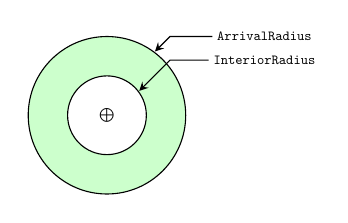
\begin{tikzpicture}
        \node[circle, minimum size=2cm, draw, fill=green!20] (1) {};
        \node[circle, minimum size=1cm, draw, fill=white] (2) {};
        \node[scale=0.5] (3) {$\bigoplus$};
        \node[scale=0.5] (4) at (2, 1) {\texttt{ArrivalRadius}};
        \node[scale=0.5] (5) at (2, 0.7) {\texttt{InteriorRadius}};
        
        \draw[-stealth] (4) -- (0.8, 1) -- (0.61, 0.81);
        \draw[-stealth] (5) -- (0.8, 0.7) -- (0.41, 0.31);
    \end{tikzpicture}
    \caption{Esquema del steering Arrive}
    \label{fig:arrive}
\end{figure}

Cuando estamos fuera de ambos radios se aplicará una velocidad máxima, con el objetivo de llegar rápido al punto. Si estamos en la región entre ambos radios se aplica una velocidad máxima escalada en función de la distancia entre los agentes.

\lstinputlisting[linerange=38-55, firstnumber=38]{\ScriptsPath/Steering/Basic/Arrive.cs}

En caso de que los agentes estén lo suficientemente cerca, es decir, dentro de la región del radio interior, se frena al agente.

\lstinputlisting[linerange=31-36, firstnumber=31]{\ScriptsPath/Steering/Basic/Arrive.cs}


Por último comprobamos sí la aceleración calculada es superior a la máxima aceleración del personaje, y en caso de ser superior la acotamos. 

\lstinputlisting[linerange=57-64, firstnumber=57]{\ScriptsPath/Steering/Basic/Arrive.cs}
